% Geometry, font
\documentclass[12pt, letter]{article}
\usepackage[margin=0.8in]{geometry}
\usepackage[T1]{fontenc}
\usepackage{fourier}
\usepackage{titling}
\setlength{\droptitle}{-5em} 
\usepackage[parfill]{parskip}
\usepackage{graphicx}
\graphicspath{{imgs/}}
\usepackage{hyperref}

% Math stuff
\usepackage{amssymb}
\usepackage{bm}

% Code Highlighting
\usepackage{minted}
\usemintedstyle{solarizedlight}

\author{Zach Neveu}
\title{ Day 18 Notes }

\begin{document}
\maketitle
\section{Agenda}%
\label{sec:agenda}
\begin{itemize}
	\item Dynamic TSP Review
	\item Local Search
\end{itemize}

\section{Dynamic TSP}%
\label{sec:dynamic_tsp}
\begin{itemize}
	\item Review concept of Hamiltonian paths $c(\bm{S},k)$
	\item To optimize $c(\bm{S},k)$, try all possible last nodes on the path before k, and choose minimum.
	\item $c(\bm{S},k) = argmin_k[c(s- \{k\}, m) + w[m,k]] } $
	\item $c(\{2\}, 2 = w[1,2]$ base case. Cheapest HP with one node is just weight of single path.
	\item $c(\{4,2\},2)=c(\{4\}, 4)+w[4,2]  $
	\item $c(\{2,4,6\} , 2) = min_k(c(\{4,6\}, 4)+w[4,2], c(\{4,6\}, 6)+w[6,2])$
	\item Once all costs are generated from 1 to all other nodes, just add paths from last node back to 1 and minimize.
	\item Problem: $O(n_2^{n})$ entries, each computation is $O(n)$, so complexity is $O(n^22^{n})$
	\item Exhaustive algorithm requires $O(n!)$
	 \item $2^{n}$ smaller than $n!$, so we actually have a good improvement!
	  \item Difference is, exhaustive algorithm re-solves all subproblems every time.
	  \item \textbf{quiz q idea}: write top down/bottom up algorithm to solve TSP this way
\end{itemize}

\section{Local Search}%
\label{sec:local_search}
\begin{itemize}
	\item "Blunt tool" that works almost everywhere
	\item Usually a heuristic, not exact
	\item Really dang good results sometimes
	\item Key idea: Good solutions lie in similar areas. If you have a good solution, try tweaking it a little to see if it gets better.
	\item Consider optimization problems in form $(F,c)$ where  $F$ is feasible set and $c$ is cost function
	\item Given a \textbf{neighborhood function} which maps each element of $F$ onto a subset $f \in F$ 
	\item Given $F$, $N(t)$, is set of feasible points "near" t
	\item \textbf{Improvement function}: \texttt{improve(t)} returns any neighbor with lower cost, or none if none exist.
\end{itemize}

\begin{minted}{Python}
# Generic Local Search Algorithm
t = rand(F) # random point in F
while improve(t) is not None:
    t = improve(t)
return t
\end{minted}

\begin{itemize}
    \item Details to Fill in:
    \begin{enumerate}
        \item How to select initial solution?
        \item How is the neighborhood defined?
        \item How to select a neighbor?
        \item What to do when there are no better neighbors? (exploration vs. exploitation dilemma)
    \end{enumerate}
    \item No single right answer, but many good options
\end{itemize}

\subsection*{Initial Solutions (TSP as example)}
\begin{itemize}
    \item Assume TSP on fully connected graph
    \item Nearest Neighbor (NN): At every step, visit closest neighbor that has not already been visited.
    \begin{itemize}
        \item Euclidean instances: 26\% from HK bound - pretty good!
        \item Non-euclidean instances: 130-410\% from HK bound - not so good
    \end{itemize}
    \item Greedy Algorithm (GD): TSP version of spanning tree. Keep adding cheapest edge, so long as it doesn't create a node of degree 3, or a cycle.
    \begin{itemize}
        \item Euglidean: 14\%-20\% of HKB
        \item Non-Euclidean: 100\%-280\% of HKB
    \end{itemize}
\end{itemize}

\subsection*{Insertion Algorithms}
\begin{itemize}
    \item All start with small tour, and add nodes such that it is always expanding
    \item Nearest Addition
    \begin{itemize}
        \item Given tour, find closest node not on tour(k) to a node on the tour (j)
        \item Select a neighbor, i, of j.
        \item Delete delete i,j, add j,k and k,i
    \end{itemize}
    \item Cheapest Insertion
    \begin{itemize}
        \item Similar to nearest addition, but minimize cost of j,k+k,i instead of just j,k
        \item Select node that minimizes c[i,k]+c[k,j]-c[i,j]
        \item Slower than nearest addition, but logically would be more accurate
    \end{itemize}
    \item Farthest Insertion
    \begin{itemize}
        \item Select node furthest from tour, then use cheapest insertion to find where to add it
        \item Euclidean: 16\% from HKB
    \end{itemize}
\end{itemize}

\subsection*{Other 2 Algorithms (category name?)}
\begin{itemize}
    \item MST vs TSP
    \begin{itemize}
        \item Deleting one edge from HC gives spanning tree!
        \item Cheapest HC must be more expensive than MST.
        \item MST is lower bound on HC cost
        \item Possible to adjust edges of MST to create HC?
        \item Traverse tree by always visiting an unvisited neighbor. Backtrack when hit a dead end.
        \item When backtracking, don't keep track of nodes that have already been visited.
        \item On example graph, go IHGEGHFDADFCFBFI, but don't record the backwards sections
    \end{itemize}
    \item Eulerian Cycle Approach
    \begin{itemize}
        \item Eulerian cycle visits each edge once.
        \item Eulerian cycle exists if each node of the graph has even degree - trivial to compute
        \item Given MST, find all nodes with odd degree
        \item Find minimum weighted matching among these odd degree nodes and add edges that are found
        \item Now an Eulerian cycle must exist!
        \item Find this, and convert it to a HC.
    \end{itemize}
\end{itemize}

\begin{figure}[h]
    \centering
    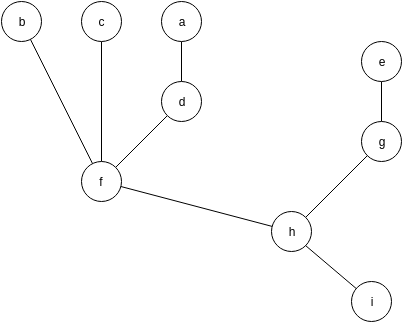
\includegraphics[width=0.6\textwidth]{exgraph}
    \caption{Example Graph}
    \label{fig:exgraph}
\end{figure}
\subsection*{Experimental Methodology}
\begin{itemize}
    \item How to compare algorithm IRL?
    \item TSPLIB - large, standard collection of hard TSP instances.
    \item Multiple reasons TSP can be hard
    \begin{itemize}
        \item For instances from real maps, a->b always shorter than or equal to a->c->b \textbf{triangle inequality} 
        \item Random graphs will not generally satisfy this
        \item Triangle inequality helps both heuristics and speed of optimal solutions
    \end{itemize}
    \item TSPLIB separated into ``euclidean"->triangle inequality holds and ``non-euclidean"->triangle inequality doesn't hold
    \item Using bounds, it is possible to get an upper limit on the difference between a heuristic value and the optimal solution.
    \item Express TSP in ILP, then use LP bound. Unfortunately, this is long, so approximates used -> Held-Karp bound.
\end{itemize}

\end{document}
